% =============================================================================
% Paper-next -- bounded signed-JSON receipt-semantics measurement
% This draft deliberately uses article layout until a human selects a venue.
% =============================================================================
\documentclass[10pt,twocolumn,letterpaper]{article}

\usepackage[margin=0.75in,columnsep=0.25in]{geometry}
\usepackage[T1]{fontenc}
\usepackage[utf8]{inputenc}
\usepackage{lmodern}
\usepackage{amsmath,amssymb}
\usepackage{array,booktabs,tabularx}
\usepackage{balance}
\usepackage{caption}
\usepackage{enumitem}
\usepackage{graphicx}
\usepackage{microtype}
\usepackage{xcolor}
\usepackage{url}
\usepackage[hidelinks]{hyperref}
\usepackage{pgfplots}
\pgfplotsset{compat=1.18}
\usetikzlibrary{positioning,arrows.meta}

\captionsetup{font=small,labelfont=bf}
\setlist{nosep,leftmargin=1.2em}
\newcolumntype{Y}{>{\raggedright\arraybackslash}X}
\newcommand{\ghostark}{Ghost-Ark}
\newcommand{\identity}{\mathsf{ID}}
\newcommand{\decision}{\mathsf{D}}
\newcommand{\raw}{\mathsf{raw}}
\newcommand{\canon}{\mathsf{canon}}
\newcommand{\admitted}{\Sigma}
\newcommand{\engines}{\mathcal{P}}

% Generated numerical anchors. Run node tools/paper-next-evidence.mjs --render
% after changing evidence-manifest.v1.json; do not hand-edit the values.
% This file is generated by tools/paper-next-evidence.mjs from evidence-manifest.v1.json.
% Do not edit it by hand; run: node tools/paper-next-evidence.mjs --render
% Values are evidence-record anchors, not population estimates unless stated in the manuscript.
\newcommand{\pnEOneClasses}{31}
\newcommand{\pnEOneUnguarded}{5}
\newcommand{\pnEOneStrict}{0}
\newcommand{\pnEOneStrictAsymmetry}{0}
\newcommand{\pnEOneBSuccesses}{403}
\newcommand{\pnEOneBDenominator}{767}
\newcommand{\pnEOneBRate}{52.5\%}
\newcommand{\pnEOneBInterval}{[49.0\%, 56.1\%]}
\newcommand{\pnEOneBStrictRate}{0.0\%}
\newcommand{\pnEOneBStrictInterval}{[0.0\%, 0.5\%]}
\newcommand{\pnESevenInputs}{1{,}500}
\newcommand{\pnESevenClasses}{8}
\newcommand{\pnESevenMechanisms}{4}
\newcommand{\pnEElevenArms}{4}
\newcommand{\pnEElevenClasses}{31}
\newcommand{\pnEElevenUnintended}{4}
\newcommand{\pnEElevenDuplicates}{3}
\newcommand{\pnETwelveDraws}{3{,}000}
\newcommand{\pnETwelveEligible}{64}
\newcommand{\pnETwelveObserved}{0}
\newcommand{\pnETwelveProducers}{16}
\newcommand{\pnETwelveControls}{7}
\newcommand{\pnEThirteenForward}{2}
\newcommand{\pnEThirteenRepairsBySeparation}{0}
\newcommand{\pnESixteenEngines}{4}
\newcommand{\pnESixteenCells}{8}


\title{\vspace{-1.4em}\textbf{One Canonical Identity, Different Policy Outcomes}\\
\large A Bounded Measurement of JSON Receipt Semantics\vspace{-0.6em}}
\author{Pranav Bhave}
\date{}

\begin{document}
\maketitle

\begin{abstract}
Signed JSON evidence commonly assigns an identity after parsing and
canonicalization.  That identity is useful only to the extent that the
distinctions it removes are irrelevant to the decisions for which the evidence
is later used.  We report a bounded measurement of that condition for a
JavaScript-style receipt canonicalizer, selected version-pinned third-party
engines, and explicitly declared adversarial inputs.  In a curated
\pnEOneClasses-class census, the unguarded receipt path collapsed
\pnEOneUnguarded{} intended distinctions; raw-text admission eliminated those
collapses in the same census.  Four external canonicalizer ecosystems each
showed \pnEElevenUnintended{} unintended members, with duplicate-key cases
shared across all four.  Under author-supplied equality policies, named
third-party engines produced \pnESixteenCells{} decision-split cells for pairs
that one receipt identity merged.  A separate, opportunity-limited sample of
\pnETwelveDraws{} Rekor index draws yielded \pnETwelveEligible{} eligible
payloads and observed no selected pathologies.  Thus the paper establishes
neither traffic prevalence nor a deployed application failure.  Its
contribution is a reproducible measurement boundary: the observed behavior is
conditioned on a canonicalizer, an admitted input alphabet, named engine
versions, and experiment-authored decisions.
\end{abstract}

\section{Introduction}
\label{sec:intro}

A digital signature binds a sequence of bytes; a receipt system often binds a
derived representation.  The difference matters when a raw JSON document is
parsed, transformed into a canonical value, and then given one digest or receipt
identifier.  If two raw documents become one identity while a downstream
decision distinguishes them, the identity is too coarse for that declared use.
This is a representation question, not a claim that signing establishes the
truth of a payload or the quality of an upstream decision.

Canonicalization and semantic divergence are established concerns.  I-JSON
limits duplicate member names and numeric representations
\cite{rfc7493}; JCS defines a canonical JSON serialization profile
\cite{rfc8785}; and the Verifiable Credential Data Integrity recommendation
discusses canonicalization and data-loss boundaries
\cite{w3c-vcdi-2025}.  Parser differentials have also been measured broadly:
Crossy tested 22 JSON parsers across languages \cite{moller2024cross}.
More generally, signed-document and multi-parser work has demonstrated that a
valid signature can coexist with divergent interpretation
\cite{rohlmann2023signature,you2025zip}.  Recent work explicitly frames
canonicality relative to downstream semantic equality
\cite{bromme2026canonicalization}.  We therefore do not present a new
canonicalization theory, a JSON-parser discovery, or a new receipt format.

Instead, we ask one constrained empirical question:

\begin{quote}
\emph{For a named receipt identity, declared input alphabet, and selected
version-pinned decision engines, do merged documents always induce the same
experiment-authored decision?}
\end{quote}

The answer in this measurement is no for selected constructions, and yes for
the E12 sampled payload slice with respect to the tested constructions.  Those
two findings must stay together.  Constructibility does not imply incidence;
a null observation in a narrow corpus does not establish absence elsewhere.

\paragraph{Contributions.}
This paper makes four bounded contributions.

\begin{enumerate}
  \item It states a decision-conditioned measurement protocol for JSON receipt
  identity, separating raw document equality, canonical identity, and a named
  downstream decision.
  \item It reports a controlled census and seeded probe for the \ghostark{}
  JavaScript-style canonicalizer, plus a selected external canonicalizer
  census.
  \item It shows concrete decision differences under author-supplied
  policy-engine executions, while explicitly separating that consequence
  census from deployed relying-party evidence.
  \item It treats a negative, opportunity-limited DSSE payload observation as
  first-class evidence and supplies an evidence binder that ties all numerical
  macros to frozen source anchors.
\end{enumerate}

\section{What is measured}
\label{sec:model}

Let $x$ be raw JSON text.  A receipt pipeline accepts $x$ only when
$x\in\admitted$, then parses and canonicalizes it to $\canon(x)$, and assigns
$\identity(x)=H(\canon(x))$.  A selected engine $p\in\engines$ executes an
author-supplied decision function $\decision_p(x)$ over the document under a
version-pinned implementation and policy.  The measurement seeks pairs
$(x,y)$ for which
\[
 x,y\in\admitted \quad\land\quad \identity(x)=\identity(y)
 \quad\land\quad \decision_p(x)\ne\decision_p(y).
\]
This notation is only a compact description of the experiment.  It does not
assert a new theorem, an exhaustive consumer model, or a property of all JSON
software.

Figure~\ref{fig:model} depicts the distinction.  A receipt identity can be
appropriate for one decision relation and too coarse for another.  The input
alphabet is equally important: rejecting ambiguous raw texts before
canonicalization can eliminate a measured collapse, while accepting a larger
alphabet can introduce one.

\begin{figure*}[t]
  \centering
  \resizebox{0.92\textwidth}{!}{% Conceptual model. The labels are grounded by E1/E16; it contains no measured rate.
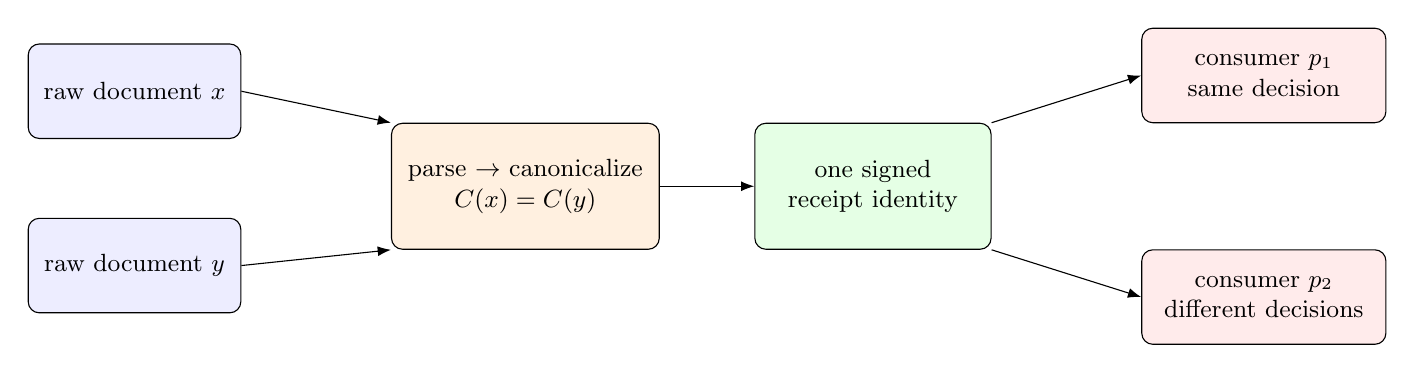
\begin{tikzpicture}[font=\small, node distance=10mm and 12mm, >=Latex]
  \node[draw, rounded corners, fill=blue!7, align=center, minimum width=27mm, minimum height=12mm] (a) {raw document $x$};
  \node[draw, rounded corners, fill=blue!7, below=of a, align=center, minimum width=27mm, minimum height=12mm] (b) {raw document $y$};
  \node[draw, rounded corners, fill=orange!12, right=of a.south east, xshift=7mm, yshift=-6mm, align=center, minimum width=34mm, minimum height=16mm] (c) {parse $\rightarrow$ canonicalize\\$C(x)=C(y)$};
  \node[draw, rounded corners, fill=green!10, right=of c, align=center, minimum width=30mm, minimum height=16mm] (r) {one signed\\receipt identity};
  \node[draw, rounded corners, fill=red!8, right=of r.north east, xshift=7mm, yshift=6mm, align=center, minimum width=31mm, minimum height=12mm] (p1) {consumer $p_1$\\same decision};
  \node[draw, rounded corners, fill=red!8, right=of r.south east, xshift=7mm, yshift=-6mm, align=center, minimum width=31mm, minimum height=12mm] (p2) {consumer $p_2$\\different decisions};
  \draw[->] (a.east) -- (c.north west);
  \draw[->] (b.east) -- (c.south west);
  \draw[->] (c) -- (r);
  \draw[->] (r.north east) -- (p1.west);
  \draw[->] (r.south east) -- (p2.west);
\end{tikzpicture}
}
  \caption{Measurement model.  The lower decision branch is an observed
  possibility in the selected experiments, not a rate or a universal
  behavior.}
  \label{fig:model}
\end{figure*}

\subsection{Boundary and threat model}

The study evaluates a local parse--canonicalize--digest path and explicit
third-party command-line or library arms.  It does not evaluate a deployed
receipt consumer, a cloud authorization path, cryptographic key custody, or
agent behavior.  An observed decision split says only that a selected engine
under a policy written for this experiment distinguishes two inputs that the
chosen receipt path merges.  It is not an observed production authorization
failure.

The adversarial corpus includes malformed or ambiguity-bearing JSON
constructions such as duplicate keys, numeric representations, and string
edge cases.  It is curated for diagnostic contrast, not sampled from ordinary
traffic.  The E12 arm is intentionally different: it samples a defined
supply-chain payload slice and searches it with controls, but its eligibility
filter leaves a small, producer-clustered denominator.

\section{Measurement design}
\label{sec:design}

\subsection{Receipt-path census and randomized probe}

E1 enumerates \pnEOneClasses{} predeclared pathology classes through the
\ghostark{} receipt path.  An unintended kernel member is a pair that
canonicalizes to the same identity despite being marked distinct by the
experiment's intended-value relation.  The unguarded arm found
\pnEOneUnguarded{} such members.  A strict raw-text admission arm found
\pnEOneStrict{} and had \pnEOneStrictAsymmetry{} rejection-asymmetry cases in
this census.

E1-B supplements the curated census with a declared seeded adversarial
generator.  The unguarded arm found \pnEOneBSuccesses{}/\pnEOneBDenominator{}
collapses (\pnEOneBRate{}, Wilson \pnEOneBInterval{}); strict admission found
$0/\pnEOneBDenominator{}$ (\pnEOneBStrictRate{}, Wilson
\pnEOneBStrictInterval{}).  These intervals describe repeated draws from that
generator, not user traffic or a general security rate.

\subsection{External canonicalizer and differential arms}

E7 generates \pnESevenInputs{} seeded inputs across V8, CPython, and jq,
finding \pnESevenClasses{} structural divergence classes over
\pnESevenMechanisms{} mechanisms.  Every pair of those selected arms disagreed
somewhere.  E11 asks a narrower portability question using \pnEElevenArms{} canonicalizer
ecosystems that this project did not author: Rust \texttt{serde\_json}, Ruby
JSON, CPython JSON, and \texttt{jq -S -c}.  Each had
\pnEElevenUnintended{} unintended members in the same
\pnEElevenClasses-class diagnostic census.  Three duplicate-key classes were
shared across all arms; no third-party arm exhibited the $2^{53}$ construction,
which confines that numeric observation to a double-backed model rather than
the JSON data format generally.

\begin{figure}[t]
  \centering
  \resizebox{\columnwidth}{!}{% Generated from figures/data/third-party-kernel.csv, extracted from E11's recorded 31-class census.
\begin{tikzpicture}
\begin{axis}[
  ybar stacked,
  width=\columnwidth,
  height=45mm,
  ymin=0, ymax=13,
  ylabel={classes},
  symbolic x coords={Rust serde-json,Ruby JSON,CPython json,jq -S -c},
  xtick=data,
  x tick label style={rotate=18,anchor=east,font=\scriptsize},
  legend style={at={(0.5,1.02)},anchor=south,legend columns=2,font=\scriptsize},
  enlarge x limits=0.14,
  bar width=8pt,
  axis line style={draw=black!55},
  tick style={draw=black!55}
]
\addplot+[fill=red!65,draw=none] table[x=arm,y=unintended_kernel,col sep=comma] {figures/data/third-party-kernel.csv};
\addplot+[fill=orange!75,draw=none] table[x=arm,y=over_discrimination,col sep=comma] {figures/data/third-party-kernel.csv};
\addplot+[fill=blue!45,draw=none] table[x=arm,y=fail_closed,col sep=comma] {figures/data/third-party-kernel.csv};
\addplot+[fill=green!50!black,draw=none] table[x=arm,y=sound_by_rejection,col sep=comma] {figures/data/third-party-kernel.csv};
\legend{unintended kernel,over-discrimination,fail-closed,sound by rejection}
\end{axis}
\end{tikzpicture}
}
  \caption{E11 diagnostic classifications across selected external
  canonicalizer arms.  Counts are census members, not ecosystem frequencies.}
  \label{fig:e11}
\end{figure}

\subsection{Decision consequence and ecological control}

E16 evaluates six curated pairs against four version-pinned engines under
author-supplied equality policies.  It records \pnESixteenCells{} engine--pair
decision splits.  The decimal-literal pair split OPA, CUE, and jq; the
$2^{53}$ pair split all four engines; CUE alone distinguished the selected
duplicate-key pair; and a trailing-zero pair supplied a same-decision
discriminator.  This establishes a selected consequence existence result.  It
does not establish that those engines consume \ghostark{} receipts or that a
deployed policy would make the same choice.

E12 supplies the counterweight.  From \pnETwelveDraws{} uniform Rekor index
draws, only \pnETwelveEligible{} \texttt{intoto} payloads were eligible for
the selected scan, spanning \pnETwelveProducers{} clustered producers.
The observed count was 0/\pnETwelveEligible{} for the tested pathologies; all
\pnETwelveControls{} detector controls fired and all eligible payload hashes
matched.  This is a constructible-but-not-observed result for an
era-skewed, opportunity-limited slice.  It is not a prevalence estimate, a
producer-level estimate, or evidence of a DSSE weakness: DSSE signs raw
payload bytes \cite{dssev1}.

\begin{figure}[t]
  \centering
  \resizebox{\columnwidth}{!}{% Generated from figures/data/ecology-consequence.csv; compare evidence classes, not rates.
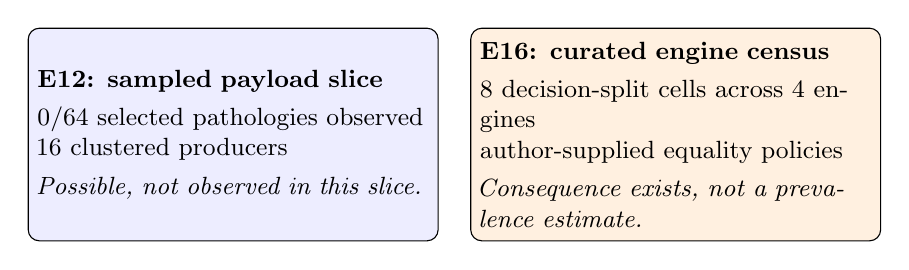
\begin{tikzpicture}[font=\small]
  \node[draw, rounded corners, fill=blue!7, align=left, text width=0.41\columnwidth, minimum height=27mm] (e12) {
    \textbf{E12: sampled payload slice}\\[1mm]
    $\pnETwelveObserved/\pnETwelveEligible$ selected pathologies observed\\
    $\pnETwelveProducers$ clustered producers\\[1mm]
    \emph{Possible, not observed in this slice.}
  };
  \node[draw, rounded corners, fill=orange!12, align=left, text width=0.41\columnwidth, minimum height=27mm, right=4mm of e12] (e16) {
    \textbf{E16: curated engine census}\\[1mm]
    $\pnESixteenCells$ decision-split cells across $\pnESixteenEngines$ engines\\
    author-supplied equality policies\\[1mm]
    \emph{Consequence exists, not a prevalence estimate.}
  };
\end{tikzpicture}
}
  \caption{Two evidence classes kept deliberately separate.  E12 is a
  sampled null observation; E16 is a curated consequence census.}
  \label{fig:e12-e16}
\end{figure}

\subsection{Composition as supporting evidence}

E13 evaluates whether a downstream stage can separate two accepted inputs
already collapsed upstream.  Its finite model covers 625 hops and 390,625
compositions, with \pnEThirteenRepairsBySeparation{} repairs by separation.
The implementation arm records \pnEThirteenForward{} forward counterexample
cells, both relying on a non-default CPython \texttt{surrogatepass} codec
before jq.  No all-default pair reproduced that implementation result.  We
therefore retain composition as supporting placement evidence rather than a
headline deployment claim.

\begin{figure}[t]
  \centering
  \resizebox{\columnwidth}{!}{% E13 supporting result: real configuration selected under a non-default permissive codec.
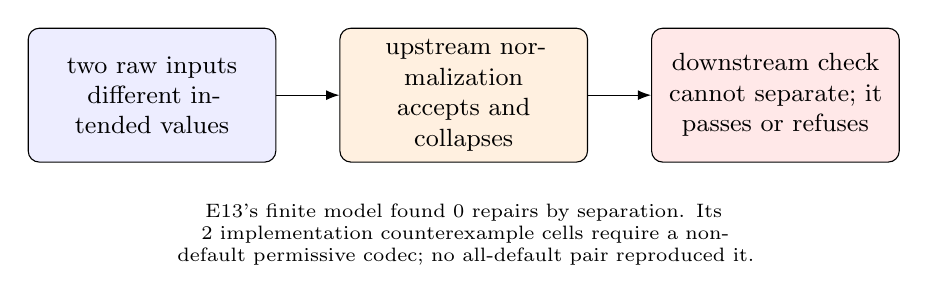
\begin{tikzpicture}[font=\small, node distance=8mm, >=Latex]
  \node[draw, rounded corners, fill=blue!7, align=center, text width=0.24\columnwidth, minimum height=17mm] (raw) {two raw inputs\\different intended values};
  \node[draw, rounded corners, fill=orange!12, align=center, text width=0.24\columnwidth, minimum height=17mm, right=of raw] (up) {upstream normalization\\accepts and collapses};
  \node[draw, rounded corners, fill=red!9, align=center, text width=0.24\columnwidth, minimum height=17mm, right=of up] (down) {downstream check\\cannot separate; it passes or refuses};
  \draw[->] (raw) -- (up);
  \draw[->] (up) -- (down);
  \node[below=4mm of up, align=center, text width=0.72\columnwidth, font=\scriptsize] {E13's finite model found $\pnEThirteenRepairsBySeparation$ repairs by separation. Its $\pnEThirteenForward$ implementation counterexample cells require a non-default permissive codec; no all-default pair reproduced it.};
\end{tikzpicture}
}
  \caption{E13's supporting placement boundary.  The reported implementation
  cells require a selected non-default codec configuration.}
  \label{fig:e13}
\end{figure}

\section{Results and interpretation}
\label{sec:results}

The measurements show three distinct facts.

\paragraph{A raw-text boundary changes the measured result.}
Within the declared pathology corpus and generator, strict admission removed
the measured unintended merges.  This is a result about that admission policy
and alphabet; it does not assert conformance to JCS, I-JSON, or any other
profile.  Standards such as I-JSON and JCS remain useful comparison points,
not properties attributed to the local implementation
\cite{rfc7493,rfc8785}.

\paragraph{The observation is not confined to one implementation.}
The E7 and E11 arms show that selected JSON ecosystems induce different
equivalence relations and that duplicate-key collapses occur in all four E11
arms.  This does not rank libraries, establish exploitability, or measure
market adoption.  It motivates recording parser, canonicalizer, and policy
versions with any receipt claim that relies on their interpretation.

\paragraph{One identity can induce different selected decisions.}
E16 connects identity collapse to a concrete decision distinction.  The
result's strength is existential and controlled: named, released engines made
different outputs under policies we authored.  Its weakness is equally clear:
there is no independently maintained receipt-relying application in the
measurement.  This is why the E12 null result is central rather than an
appendix footnote.

\section{Relation to prior art}
\label{sec:related}

The closest conceptual prior work is Brömme's treatment of canonicalization
failure as representation divergence relative to relevant semantic equality
\cite{bromme2026canonicalization}.  Our delta is not a new semantic-equality
criterion.  It is the bounded package of (i) a receipt-path identity
measurement, (ii) version-pinned decision executions, and (iii) an ecological
null arm reported alongside selected counterexamples.

Cross-language JSON testing already supplies broader parser-differential
coverage \cite{moller2024cross}.  We use differential behavior only as a
diagnostic component of a receipt-identity study.  Similarly, semantic gaps
between signed document consumers \cite{rohlmann2023signature} and archive
parsers \cite{you2025zip} rule out a general signature-versus-semantics
novelty claim.  We do not claim one.

Standards and format work also constrain the scope.  JCS and I-JSON give
existing JSON representation profiles \cite{rfc8785,rfc7493}; the W3C data
integrity work treats transformation-related data loss as a design concern
\cite{w3c-vcdi-2025}; EverParse demonstrates mechanically checked
parser/serializer methods for authenticated formats
\cite{ramananandro2019everparse}.  The independent Vaara Receipt draft
occupies nearby recomputable-receipt territory
\cite{sirkkavaara2026vaara}.  These works strengthen the case for narrow
measurement language, not a new receipt architecture claim.

\section{Evidence provenance}
\label{sec:artifact}

The paper is intentionally isolated from the repository's existing
transaction-control manuscript.  Its source anchors are the annotated
\texttt{evidence-v1} and \texttt{v1.0.0} revisions recorded in
\texttt{evidence-manifest.v1.json}.  The
\texttt{paper-next-evidence} gate verifies that those tags still resolve,
that each documented experiment heading exists at the frozen evidence
revision, that generated numerical macros match
\texttt{evidence-manifest.v1.json}, and that required citations resolve.

The gate does not replay E12, E13, or E16.  Their generated reports are ignored
local artifacts rather than files in the tagged release.  Exact results are
therefore tied to the frozen experiment record and source anchors, with this
limitation exposed rather than silently converting local output into a release
bundle.  This is a reproducibility aid, not independent replication.

\section{Limitations and the decisive next experiment}
\label{sec:limits}

The evidence is bounded in five ways.  First, the pathology corpus is curated.
Second, E1-B's confidence intervals are conditional on its declared generator.
Third, E11 covers four selected external arms, not their ecosystems.  Fourth,
E12 has 64 eligible payloads from 16 clustered producers and does not create a
traffic denominator for every pathology.  Fifth, E16's policies and equality
rules were authored for the experiment, and its report does not record a
usable host identifier.

The result is therefore unsuitable as a main-track systems or agent-governance
paper on the frozen artifact alone.  The single experiment most likely to
change that assessment is preregistered measurement of one independently
maintained signed structured-data ecosystem with an actual
canonicalization--reparse boundary, versioned external consumers, a
strict-rejection control, and producer-aware population accounting.  The
target should not be DSSE itself: its raw-byte signing model makes E12 a corpus
arm, not a target weakness.

\section{\quad Conclusion}

For the selected JSON receipt path, one canonical identity can cover two raw
documents that named engines distinguish under author-supplied policies.  The
same study found none of its selected constructions in a limited DSSE payload
slice.  These are jointly useful facts: they locate a representation boundary
without promoting a curated counterexample into a prevalence claim.  A receipt
claim should name the canonicalizer, accepted alphabet, and downstream
decision relation that its identity is intended to preserve.

\balance
\begingroup
\small
\setlength{\itemsep}{0pt}
\bibliographystyle{plain}
\bibliography{references}
\endgroup
\end{document}
